\documentclass[12pt,letterpaper,english,bibliography=totocnumbered, abstract=on]{scrartcl}

\usepackage{indentfirst}
\usepackage[titletoc]{appendix}
\usepackage{fullpage}
%\usepackage{subfiles}
\usepackage[T1]{fontenc}
\usepackage[latin9]{inputenc}
\usepackage{color}
\usepackage{babel}
\usepackage{verbatim}

\usepackage{listings}
%\lstset{
%	basicstyle=\small\ttfamily,
%	columns=flexible,
%	breaklines=true
%}

\usepackage[unicode=true,pdfusetitle,
bookmarks=true,bookmarksnumbered=false,bookmarksopen=false,
breaklinks=true,pdfborder={0 0 0},pdfborderstyle={},backref=false,colorlinks=true]
{hyperref}
\hypersetup{linkcolor=blue,citecolor=blue,urlcolor=blue}

\usepackage{booktabs}
\usepackage{multirow}
\usepackage{adjustbox}
\usepackage{threeparttable}
\usepackage[table]{xcolor}
\usepackage{csquotes}
\usepackage{soul} % for hiliting text: \hl

\usepackage[backend=biber, style=authoryear, maxbibnames=99, dashed=false]{biblatex}
\setlength\bibitemsep{2\itemsep}
%\addbibresource{mylibrary.bib}
%\addbibresource{CRB.bib}

\usepackage{pdfpages}
\usepackage{float} % Allows use of H to place floats

\usepackage{pgfgantt}

\usepackage{framed}

% Prevent page breaks within paragraphs
% https://tex.stackexchange.com/questions/21983/how-to-avoid-page-breaks-inside-paragraphs
\widowpenalties 1 10000

\begin{document}

\titlehead{Technical Report}

\title{Monitoring \textit{Aulacaspis yasumatsui} on \textit{Cycas micronesica} in the Tinian Conservation Plots using Leaf Samples}

\author{Aubrey Moore and Jason Andrew}

\date{
	March 24, 2022, Revised April 2, 2022
	\footnote{
		The most recent version of this document may be downloaded from \url{https://github.com/aubreymoore/Tinian-CAS/raw/main/reports/leaf_samples.pdf}.
		
		All data and code used in this report are available in a public GitHub repository at
		\url{https://github.com/aubreymoore/Tinian-CAS}.
	}
}

\maketitle
%\footnote{\url{https://github.com/aubreymoore/2020-FS-CRB-biocontrol-project/blob/master/combined-proposal.pdf}}


\begin{abstract}
Leaf samples were collected from 12 \textit{Cycas micronesica} plants growing in the Tinian conservation plots on 2022-02-26.
The primary purpose of theses samples was to assess the presence of \textit{Aulacaspis yasumatsui}, cycad aulacaspis scale (CAS). A secondary objective was to confirm identity of the scale insect and a third objective was to look for signs of predation and/or parasitism. 

Microscopic examination indicated that the 10 most northerly sampled plants were infested with CAS. However, the 2 most southerly plants were infested only with an unidentified, dark colored armored scale (Diaspididae). Specimens of both scale insects were sent to the USDA Systematic Entomology Laboratory for species determination. No indication of predation or parasitism was seen.  
\end{abstract}



\clearpage
\tableofcontents

\clearpage
\section{Methods}

On 2022-02-26 \textit{Cycas micronesica} leaflet samples were collected at 12 points along a north-south transect of the Tinian conservation plots. This was not a random sample because the objective was to collect 2 to 4 leaflets which were most heavily infest with scale insects at each point. Leaflets were collected into vials containing food-grade propylene glycol as a preservative. Ethanol would normally be used for this, but we used propylene glycol as an alternative to avoid problems with shipping hazardous material on aircraft. The label on each vial contained a plot ID and a plant ID. Coordinates for each sampled plant were extracted the project GIS database in UTM format (Coordinate Reference System: EPSG:32655 - WGS 84 / UTM zone 55N).

After the samples were transported from Tinian to Guam, they were examined under a dissecting microscope to determine presence of scale insects, predators and parasitoids.  

Raw data were stored in a CSV file (Appendix \ref{leaf_samples.csv}) and QGIS was used to map results (Fig. \ref{fig:map-image}). 

\section{Results}

Leaflets in all samples were infested with scale insects (Figure \ref{fig:map-image}). The 10 most northerly sampled plants were infested with what appeared to be CAS. However, the 2 most southerly plants were infested with an unidentified, dark colored armored scale (Diaspididae). Specimens of both have been sent to the USDA Systematic Entomology Laboratory for species determination. This document will be updated when species determination results are received.

No indication of predation or parasitism was seen in any of the samples. 


%\begin{table}[h!]
%	\caption{Listing 1: \textbf{leaf\_samples.csv}}
%	\label{leaf_samples.csv}	
%	\lstinputlisting[basicstyle=\small\ttfamily, breaklines=true, columns=flexible]{../leaf_samples/leaf_samples.csv}
%\end{table}

% TODO: \usepackage{graphicx} required
\begin{figure}[h!]
	\centering
	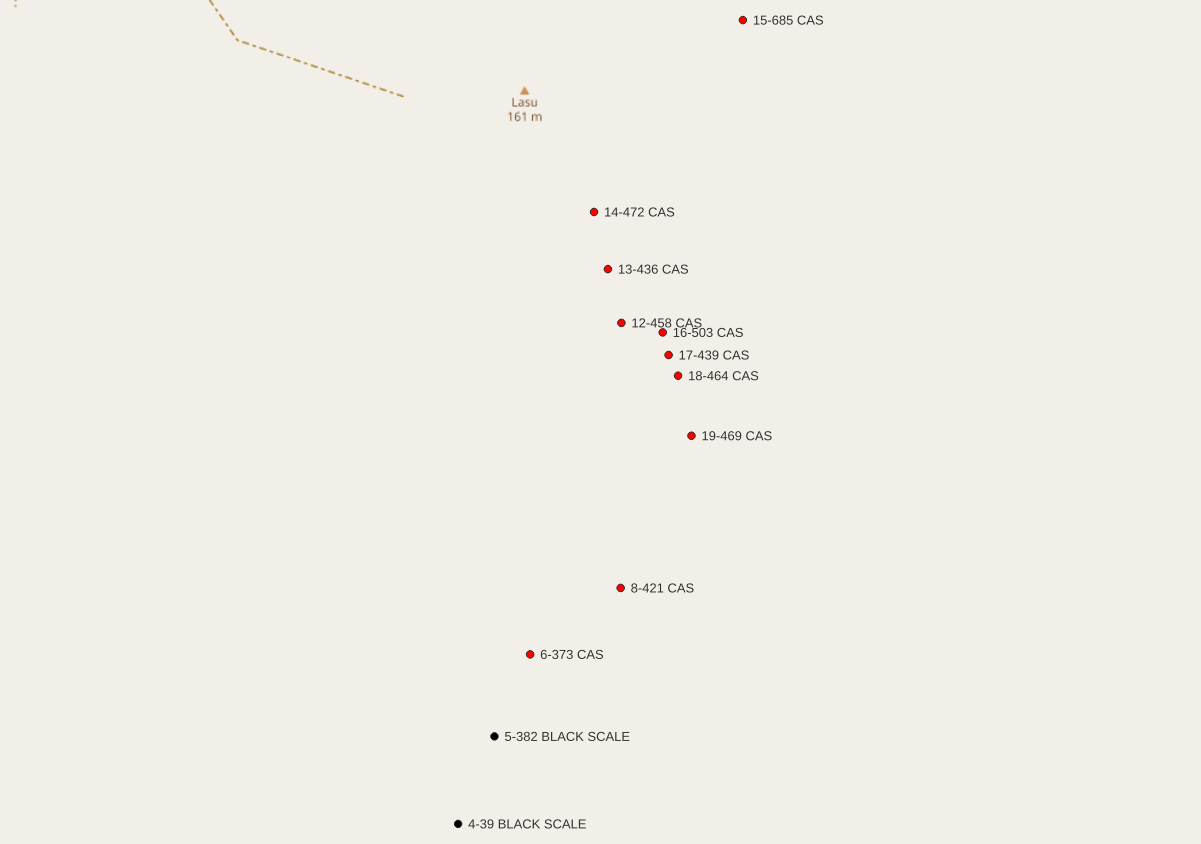
\includegraphics[width=\linewidth]{../leaf_samples/map-image}
	\caption{Map showing location of leaf samples from \textit{Cycas micronesica} growing in the Tinian conservation plots. Numbers indicate plot ID and plant ID. \textbf{CAS} indicates presence of \textit{Aulacaspis yasumatsui} on the leaf sample and \textbf{BLACK SCALE} indicates presence of an unidentified diaspidid.}
	\label{fig:map-image}
\end{figure}

\clearpage
\begin{appendices}
	
	\section{Raw data: leaf\_samples.csv}
	\label{leaf_samples.csv}
	\lstinputlisting[basicstyle=\small\ttfamily, breaklines=true, columns=flexible]{../leaf_samples/leaf_samples.csv}
		

	\section{Bibtex record}
	\begin{lstlisting}[basicstyle=\small\ttfamily, breaklines=true, columns=flexible]
	@misc{moore-2022-04-02,
	title = {Monitoring \textit{Aulacaspis yasumatsui} on \textit{Cycas micronesica} in the Tinian Conservation Plots using Leaf Samples},
	author = {Aubrey Moore and Jason Andrew},
	url = {https://github.com/aubreymoore/Tinian-CAS/raw/main/reports/leaf_samples.pdf} 	
	}
	\end{lstlisting}
		
\end{appendices}

\end{document}
